\section{Summary} 
In this thesis, we presented two new Gray codes for generating Catalan objects in cool-lex orders and loopless implementations of each of these Gray codes.  Chapter \ref{chap:otree-graycode} introduced the first pop-push Gray code for generating ordered trees.  Chapter \ref{chap:otree-implementation} provided two loopless implementations of the ordering given in Chapter \ref{chap:otree-graycode}, constituting the first fully published loopless algorithms for generating ordered trees via a pointer-based representation.  Chapter \ref{chap:luka-graycode} gives a shift Gray code for generating Łukasiewicz words with fixed content using a single left-shift per generated string. Chapter \ref{chap:luka-implementation} gives loopless implementation of the ordering in Chapter \ref{chap:luka-graycode} using a linked list representation of Łukasiewicz words for the general case and a simplified array based implementation for the special case of Motzkin words.

\section{Open Problems}

The results of this thesis have many natural extensions.  For example, Chapters \ref{chap:otree-graycode} and \ref{chap:otree-implementation} examine the cool-lex order for ordered trees. One could imagine generating other Catalan objects in cool-lex order and extending the simultaneous Gray code for Dyck words, binary trees, and ordered trees to more Catalan objects.  For example, what the ordering generated by the Gray code in Chapter \ref{chap:otree-graycode} look like if translated to the polygon triangulations seen in Chapter \ref{chap:catalan}?  What would it look like translated to fixed-length (not fixed content) Łukasiewicz words, or other Catalan objects? We leave this question as an exercise to the reader.  

Another area of extension for the ordered trees result is the pursuit of a simpler Gray code. The Gray code in Chapter \ref{chap:otree-graycode} uses either one or two pulls per generated tree.  Whether a single pull Gray code for ordered trees exists is an open problem.  

The loopless algorithm for generating Łukasiewicz words given in Section \ref{sec:luka_ll} could almost certainly be simplified.  In particular, an implementation that uses a singly linked list instead of a doubly linked list  is likely possible.  This would mirror the singly linked list implementation for looplessly generating multiset permutations by Williams \cite{williams2009loopless}, discussed in Section \ref{sec:coolPerms}.

\begin{figure}
\begin{center}
        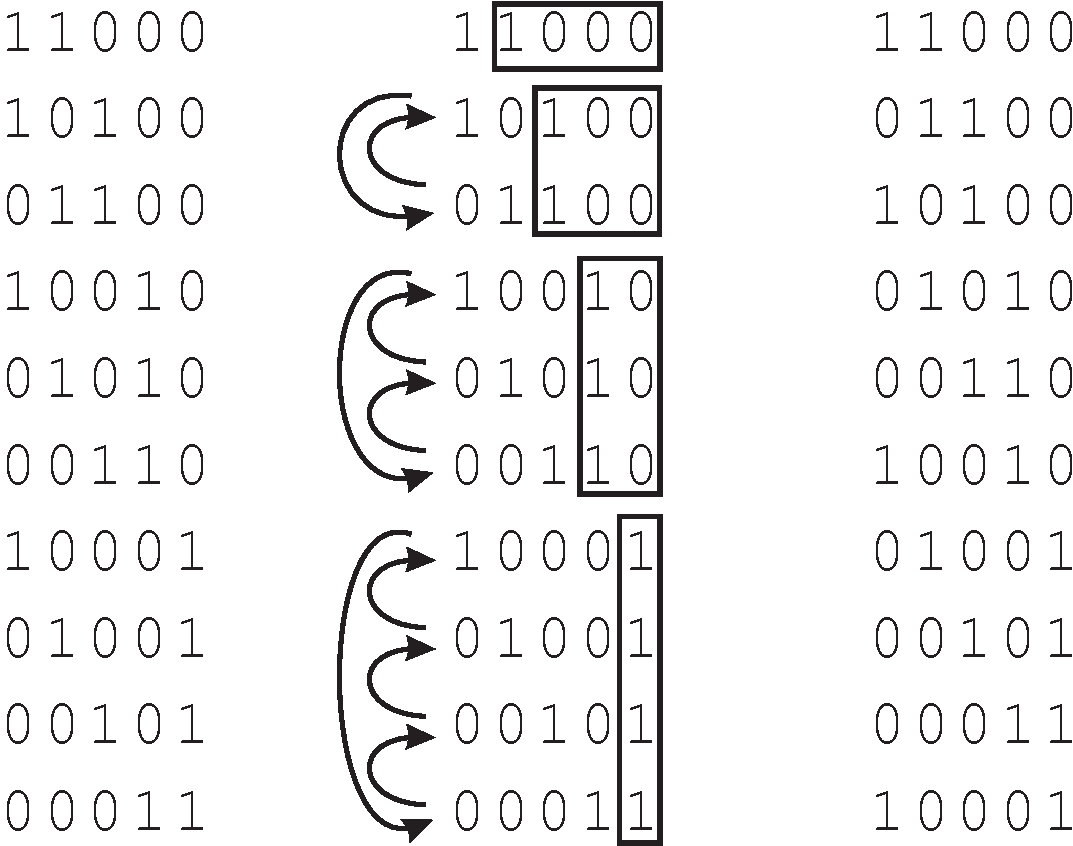
\includegraphics[width=3.5in]{transform.pdf}
\end{center}
        \cprotect\caption[Cool-lex order constructed from upward rotations of sublists of co-lexicographic order.]{Cool-lex order constructed from upward rotations of sublists of co-lexicographic order.  More precisely, the strings with a given scut are all moved up one position cyclically.  This image is taken from \cite{ruskey2005generating,ruskey2009coolest}, which introduced cool-lex order for binary strings. }
\label{fig:cooltransform}
\end{figure}

A further avenue for extension is generalizations of the recursive structure of cool-lex order.  As was discussed in Section \ref{sec:GraySublists}, the binary reflected Gray code has many sublists that are also Gray codes.  Beyond this, the idea of reversing sublists of the Gray code has been used in other Gray codes that are not sublists of the binary reflected Gray Code.  In particular, Eades and Mckay gave a modification of the binary reflected Gray code which divided strings into 3 recursive cases to generate a homogenous transposition Gray code for $(s,t)$-combinations. This ordering has a stronger closeness property than generating $(s,t)$ combinations via a sublist of the binary reflected Gray code: successive strings differ by transpositions where bits between the transpositions are all zero.  Similarly to the Eades-Mckay modification of the binary reflected Gray code, one could move past sublists of cool-lex order into generalizing the recursive structure of the order.  To understand this idea, Figure \ref{fig:cooltransform} shows how co-lexicographic order is transformed into cool-lex order via sublist rotations.  More generally, one could consider generating new ordering by breaking lists down into other sublists and upwardly rotating some of those sublists. In other words, one could look for orders that are cooler than cool. 
